\documentclass[10pt,twocolumn]{article}
\usepackage[margin=0.8in]{geometry}
\usepackage{graphicx,booktabs,amsmath,hyperref}
\title{Does Timing Matter? Temporal Signals and Time-Robustness in AI Detection of Mental-Health Risk from Reddit Posts}
\author{Group 2, COMP 8790 Topics in Applied AI \\ \small Phase I report (draft)}
\date{}
\begin{document}
\maketitle
\begin{abstract}
Saeed and Ahmed~\cite{saeed} report that adding posting-time features to a BiLSTM text classifier improves six-way classification of mental-health subreddits (weighted F1 0.7376 versus 0.7222). We test that claim against a strong text-only baseline (TF-IDF with logistic regression) and a fine-tuned MentalRoBERTa, using five replicates, paired bootstrap intervals, and a time-shift split that avoids a data-collection artefact we found in the shared dataset. For TF-IDF and the BiLSTM we find no reliable gain from time features on the paper's own random split, a gain of at most 0.006 macro F1 for the weaker BiLSTM on two splits, and a small loss for TF-IDF under time shift. MentalRoBERTa is the strongest text model (macro F1 about 0.68) and time features add nothing to it (change $-0.002$ to $0.000$, intervals include zero). Training on earlier posts and testing on later ones costs no measurable accuracy over Nov 2021 to Nov 2022.
\end{abstract}

\section{Introduction}
Reddit communities are used to study mental-health language at scale, and detection models could support triage tools. A recent paper claims that when a post was written (hour, weekday, month) carries useful signal. If true it is cheap to add, if false it may be a shortcut that breaks when data drift. We ask whether the claim holds against a strong text baseline and how each method behaves when trained on earlier posts and tested on later ones. Posts are labelled by subreddit, not by clinical diagnosis, so this is a study of community language and not of diagnosis.

\section{Problem Definition}
Given a post $x$ with text and a timestamp, predict one of six classes (depression, anxiety, bipolar, BPD, schizophrenia, mentalillness). \textbf{RQ1:} do posting-time features significantly improve macro F1 over a strong text-only model, and how much does each method lose when trained on earlier posts and tested on later ones? Our main metric is macro F1, because it weights small classes equally. We also report weighted F1 to compare with the paper, whose recall equals its accuracy, which is what weighted averaging gives.

\section{Related Work}
Our group reviewed ten papers (Table~\ref{tab:lit}). \textbf{Anchor.} Saeed and Ahmed~\cite{saeed} fuse a BiLSTM text branch with an LSTM over six time features through cross-modal attention and report weighted F1 0.7376 against 0.7222 for text only, from one split, with no transformer baseline and no code. \textbf{Simple baselines and time.} Low et al.~\cite{low} classify mental-health subreddits with TF-IDF and linear models (weighted F1 0.851) and show language changing during COVID-19, which gives us both a baseline and a pre- versus mid-COVID dataset. Cohan et al.~\cite{cohan} build SMHD and find TF-IDF models precise but low in recall, and never split by time. \textbf{Temporal models.} Kumar et al.~\cite{kumar} turn a user's post history into a time series and show that order matters at the user level, which is a different use of time from timestamps. \textbf{Evaluation.} The eRisk 2025 overview~\cite{erisk} and the DS@GT entry~\cite{dsgt} show that high recall alone is not useful (recall 1.00 with F1 0.20) and that early-detection metrics need care. \textbf{Strong text models.} MentalRoBERTa~\cite{ji} is pretrained on mental-health Reddit and is the strong text model the anchor paper never compared with; Menta~\cite{menta} shows small models can be competitive. \textbf{Methodology.} Cao et al.~\cite{cao} review 47 studies and find frequent leakage, untuned baselines and accuracy-only reporting, and Kamarudin et al.~\cite{kamarudin} survey data and methods in the field. \textbf{Gap.} No study tests whether timestamp features help once a strong text model and repeated, leakage-controlled, time-aware evaluation are used.

\begin{table*}[t]\centering\small
\begin{tabular}{p{3.0cm}p{4.3cm}p{4.2cm}p{4.5cm}}\toprule
Paper (reviewer) & Approach & Finding & Limitation \\\midrule
Saeed \& Ahmed 2025 (Abhinav) & BiLSTM + time LSTM, cross-modal attention & +1.5 F1 from time & one split, no transformer, no code \\
Low et al.\ 2020 (Sudesh) & TF-IDF/LIWC + linear models & weighted F1 0.851; COVID language shift & no transformer, post level only \\
Cohan et al.\ 2018 (Jaskamal) & SMHD, TF-IDF, FastText, CNN & high precision, low recall & no time split, data under agreement \\
Kumar et al.\ 2024 (Zohaib) & post history as a time series & order of posts matters & user level, baselines copied \\
Parapar et al.\ 2025 (Xing) & eRisk shared tasks & best F1 0.85; recall alone misleads & no timestamp features, no later-period test \\\bottomrule
\end{tabular}
\caption{The five core papers. Supporting papers: MentalBERT (Abhinav), Cao et al.\ (Sudesh), Kamarudin et al.\ (Jaskamal), Menta (Zohaib), DS@GT (Xing).}\label{tab:lit}
\end{table*}

\section{Methodology}
\paragraph{Data.} The Kaggle ``Mental Disorders Identification (Reddit)'' file (701,787 posts, 2010 to 2022, timestamps with hour, no author column) is the anchor paper's data. After the same filters (2021 and 2022 only, no NSFW, no empty or very short posts) and our leakage control, 483,715 posts remain. Leakage control removes subreddit mentions (``r/depression'', ``this sub''), texts that appear under more than one label, and duplicates. Condition names stay in the text, which makes the task easier than real detection and is a limitation. Each replicate draws a stratified 60k sample by label and month.
\paragraph{Splits.} \texttt{random} (80/20 stratified, as in the paper), \texttt{random\_matched} (same test, training reduced to the size of the time split), \texttt{temporal\_late} (train Nov 2021 to Jun 2022, test Aug to Nov 2022), and \texttt{temporal\_2021\_22} (train 2021, test 2022). The last is confounded: in this file depression, bipolar and schizophrenia posts essentially start in Nov 2021 (Fig.~\ref{fig:mix}), so it tests a collection change and not language drift. We therefore use \texttt{temporal\_late} as the valid shift test. Comparing it with \texttt{random\_matched} separates the effect of time from the effect of less training data.
\paragraph{Methods.} \textbf{A:} TF-IDF (1 to 2 grams, 50k features) with class-weighted logistic regression, $C$ tuned on a validation set. \textbf{B:} MentalRoBERTa fine-tuned with the \texttt{[CLS]} vector, 128 tokens, 2 epochs, 20k training subsample. \textbf{C:} the anchor paper's BiLSTM with an LSTM time branch and shared attention, rebuilt from its equations (embedding 128, BiLSTM 64, dropout 0.6, RMSprop). Each method is run with text only and with text plus time features (month, day, weekday, weekend, hour, working hour); C also has a concatenation variant. A design check shows the BiLSTM can memorise 300 posts.
\paragraph{Statistics.} A replicate is a fresh sample, split and model initialisation (five replicates). Differences use a paired bootstrap of test posts (1000 resamples); models are compared with McNemar's test.

\section{Data Preparation Ablations}
We also tested whether our preparation steps change the score (Method A, 20k posts, five replicates). Keeping subreddit mentions, duplicates and cross-posts, or both, gives macro F1 0.620 to 0.624 against 0.620 with full cleaning, within noise, because leakage is only about 3\% of posts. The cleaning therefore protects validity and does not raise the score. Scored on one common random reference set, label-by-month stratified and plain random samples both reach 0.623 to 0.624, while a class-balanced sample reaches 0.607 on the real class mix. Stratification mainly guarantees that every class and month is present for the time splits.

\section{Reproduction of the Anchor Paper}
Table~\ref{tab:repro} compares weighted F1 on the random split. Our BiLSTM matches the paper's text-only level but not its gain from time.
\begin{table}[h]\centering\small
\begin{tabular}{lcc}\toprule & Paper & Ours (C) \\\midrule text only & 0.7222 & 0.7302 \\ text + time & 0.7376 & 0.7296 \\\bottomrule\end{tabular}
\caption{Weighted F1, random split. Ours is the mean of five replicates.}\label{tab:repro}
\end{table}
Possible causes of the gap, all choices we had to make because no code was released: no stopword removal or lemmatisation, learned embeddings instead of Word2Vec, time features fed as a length-6 sequence, early stopping on a separate validation set (the paper selects on the reported set), and a different sample. All are logged in \texttt{logs/decision\_log.md}.

\section{Comparative Experiments}
\begin{table}[h]\centering\small
\begin{tabular}{llccc}\toprule Model & Features & random & matched & late \\\midrule
A & text & .642 & .636 & .636 \\ A & text+time & .643 & .633 & .620 \\
C & text & .630 & .609 & .608 \\ C & text+time & .630 & .614 & .614 \\
B & text & -- & .671 & .679 \\ B & text+time & -- & .671 & .677 \\\bottomrule\end{tabular}
\caption{Macro F1, mean of five replicates (B: three, not run on the random split).}\label{tab:main}
\end{table}
McNemar's test favours A over C on \texttt{random\_matched} and \texttt{temporal\_late} ($p<0.001$) and C over A on \texttt{random} by a small margin ($p=0.002$).

\section{Research Question: Does Timing Help?}
\begin{figure}[h]\centering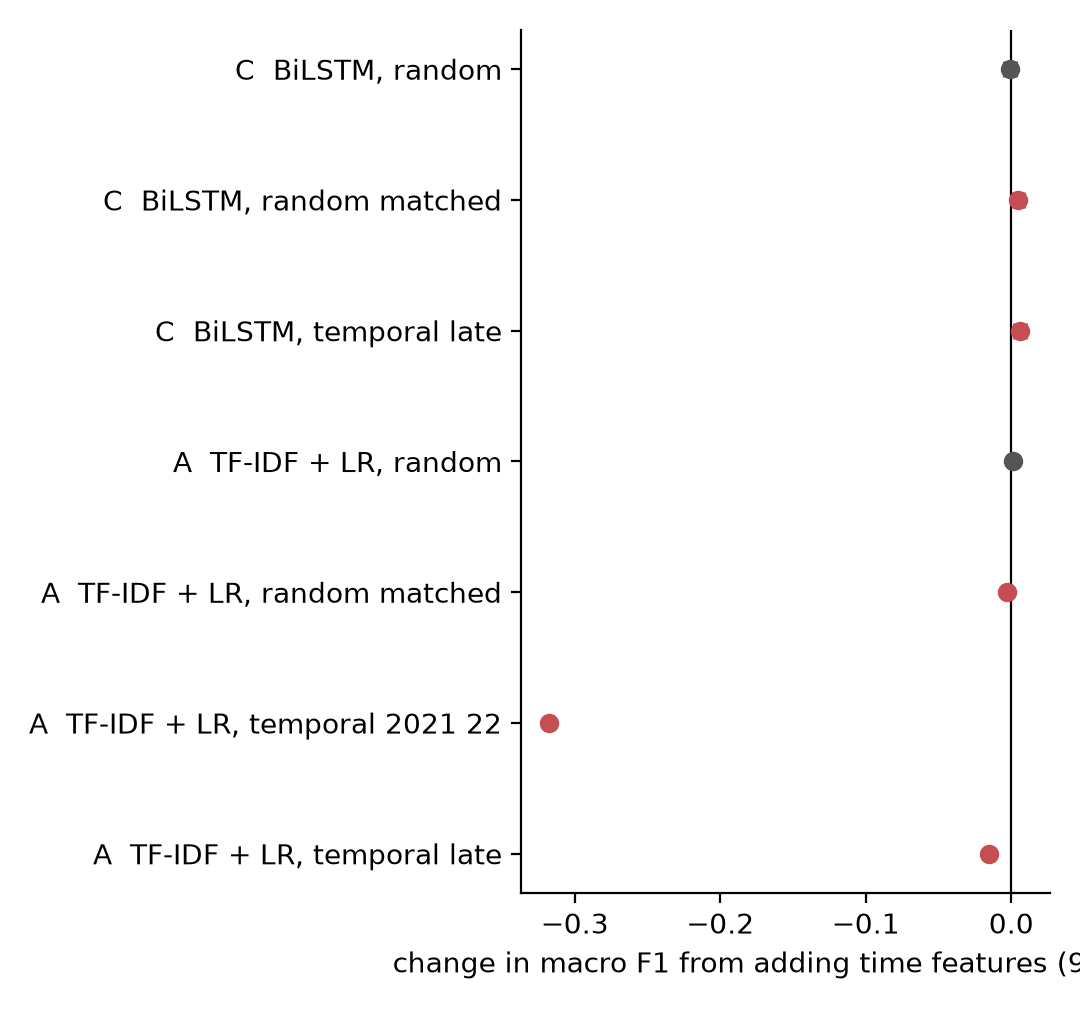
\includegraphics[width=\columnwidth]{fig2_delta_time.png}\caption{Change in macro F1 from adding time features, 95\% bootstrap interval.}\label{fig:delta}\end{figure}
On the random split every interval includes zero. For A the change is $-0.003$ on \texttt{random\_matched} and $-0.016$ on \texttt{temporal\_late}, so time hurts under shift. For C with attention the change is $+0.005$ and $+0.006$ (intervals exclude zero but are about half a point), and concatenation gives no gain. For MentalRoBERTa it is $0.000$ [$-0.003$, $+0.003$] and $-0.002$ [$-0.005$, $+0.001$]. Time alone scores 0.15, the uniform random-guess level (0.145). Posting-time features therefore do not add reliable signal over text.

\section{Extension Experiment: Time Robustness}
Macro F1 on \texttt{temporal\_late} minus \texttt{random\_matched}, text only, is $-0.001$ [$-0.008$, $+0.005$] for C, $-0.001$ [$-0.007$, $+0.006$] for A and $+0.008$ [$-0.001$, $+0.017$] for B, so training on earlier posts costs nothing measurable over these months. The confounded 2021 to 2022 split looks much worse: A with time features falls to 0.248, and to 0.543 when month and day are removed, because month features learn the class mix of 2021 (Fig.~\ref{fig:shift}).
\begin{figure}[h]\centering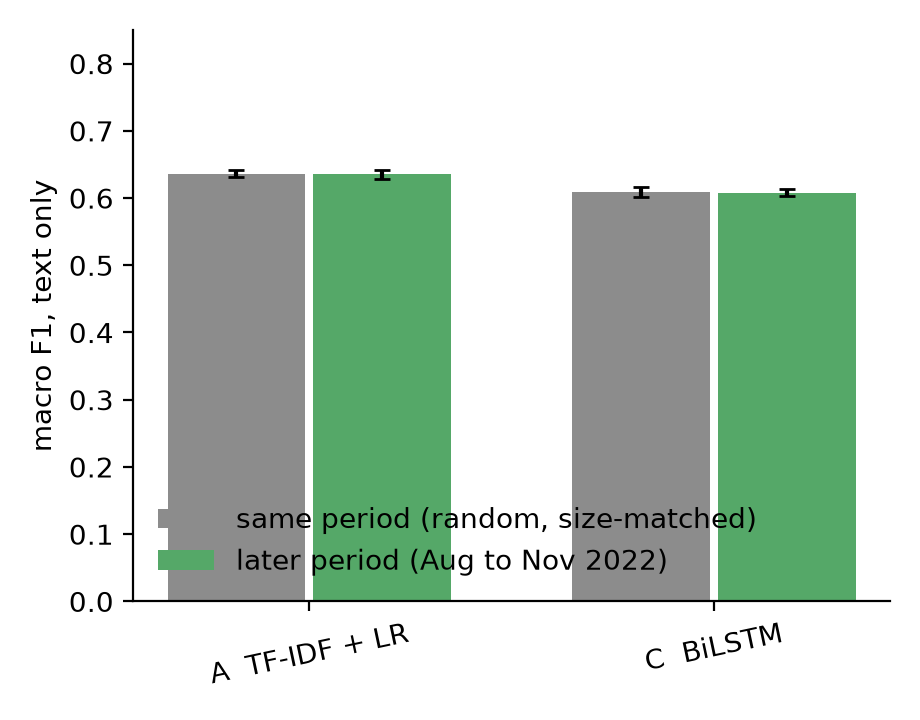
\includegraphics[width=\columnwidth]{fig3_time_shift.png}\caption{Same-period versus later-period macro F1.}\label{fig:shift}\end{figure}
\begin{figure}[h]\centering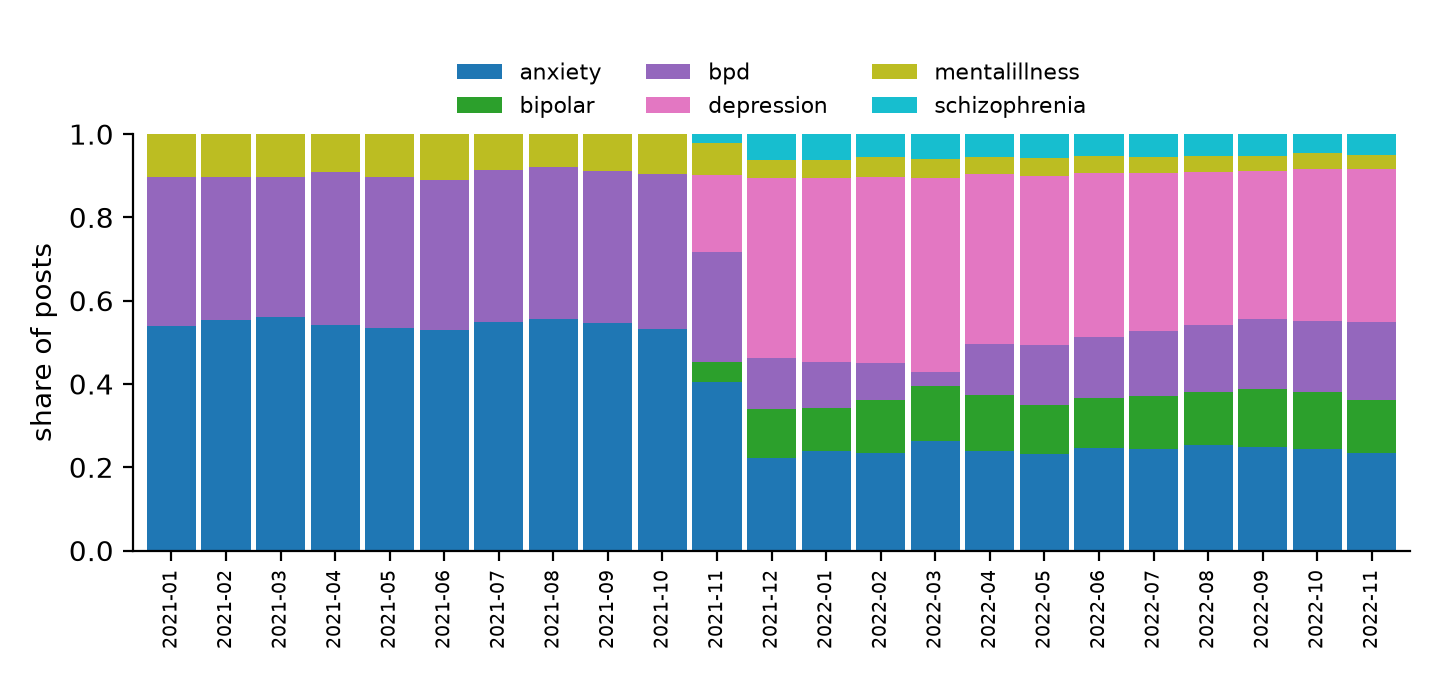
\includegraphics[width=\columnwidth]{fig4_class_mix_by_month.png}\caption{Class share by month: three classes only exist from Nov 2021.}\label{fig:mix}\end{figure}

\section{Results and Analysis}
The strongest text model is the pretrained MentalRoBERTa (about 0.68 macro F1 against 0.64 for TF-IDF and 0.61 for the BiLSTM), and time features add nothing for it. The BiLSTM's small gain may come from time acting as a weak regulariser for a weaker text encoder, which we have not tested. Errors concentrate in the small and noisy classes, mainly mentalillness (Fig.~\ref{fig:conf}).
\begin{figure}[h]\centering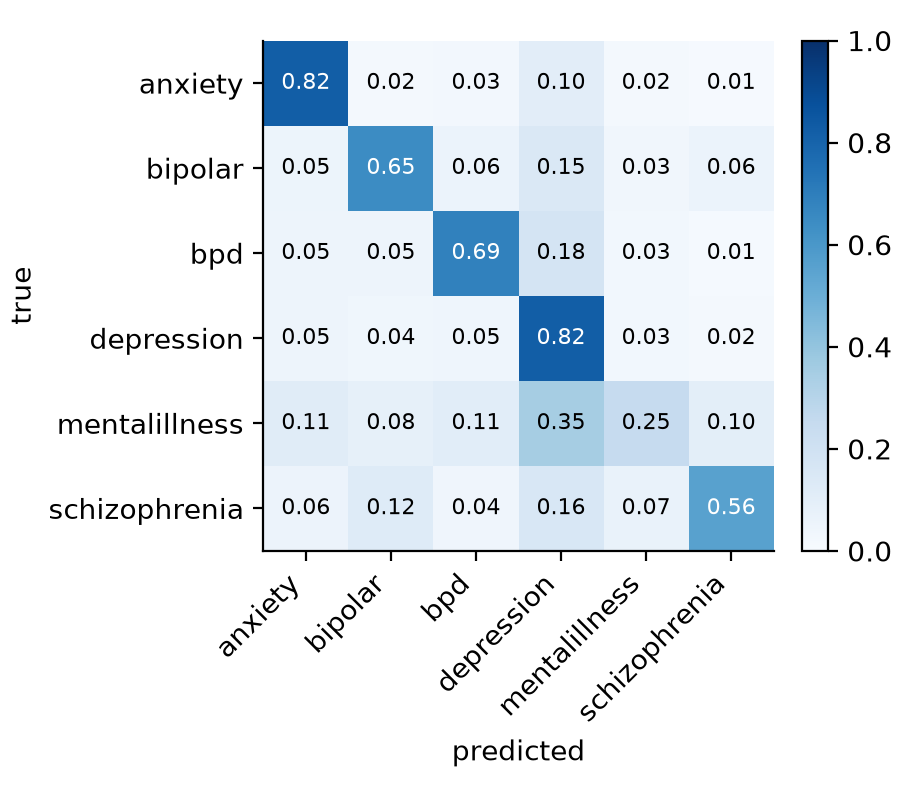
\includegraphics[width=0.8\columnwidth]{fig5_confusion_A_temporal_late.png}\caption{Method A, text only, \texttt{temporal\_late}.}\label{fig:conf}\end{figure}

\section{Limitations}
Labels are subreddits and not diagnoses. Condition names remain in the text. The Kaggle file has no author column, so same-user leakage cannot be checked there (it is checked on the Zenodo data). Method C is our rebuild. Method B uses a 20k training subsample and three replicates on two splits because of free GPU limits, so cross-method gaps partly reflect training size. The valid shift window is short (about nine months).

\section{Research Findings}
(1) The anchor paper's timing gain is not reproduced against a strong text baseline. (2) Time features can hurt under time shift. (3) No measurable loss from training on earlier posts within Nov 2021 to Nov 2022. (4) The 2021 to 2022 split used by the paper is confounded by a collection change.

\section{Conclusion}
Timing does not reliably matter for classifying these subreddits once a strong text model is used, and claims of timing gains should be checked on splits that avoid collection artefacts.

\begin{thebibliography}{10}
\bibitem{saeed} Q.~B. Saeed and I.~Ahmed. Early detection of mental health issues using social media posts. arXiv:2503.07653, 2025.
\bibitem{low} D.~M. Low, L.~Rumker, T.~Talkar, J.~Torous, G.~Cecchi, and S.~S. Ghosh. Natural language processing reveals vulnerable mental health support groups and heightened health anxiety on Reddit during COVID-19. JMIR 22(10):e22635, 2020.
\bibitem{cohan} A.~Cohan, B.~Desmet, A.~Yates, L.~Soldaini, S.~MacAvaney, and N.~Goharian. SMHD: A large-scale resource for exploring online language usage for multiple mental health conditions. COLING, 2018.
\bibitem{kumar} R.~Kumar, K.~Maharaj, A.~Saxena, and P.~Bhattacharyya. Mental disorder classification via temporal representation of text. Findings of EMNLP, 2024.
\bibitem{erisk} J.~Parapar, A.~P\'erez, X.~Wang, and F.~Crestani. Overview of eRisk at CLEF 2025: Early risk prediction on the internet. CEUR-WS 4038, 2025.
\bibitem{dsgt} A.~Miyaguchi, D.~Guecha, Y.~Chiu, and S.~Gaur. DS@GT at eRisk 2025. arXiv:2507.10958, 2025.
\bibitem{ji} S.~Ji, T.~Zhang, L.~Ansari, J.~Fu, P.~Tiwari, and E.~Cambria. MentalBERT: Publicly available pretrained language models for mental healthcare. LREC, 2022.
\bibitem{cao} Y.~Cao et al. Machine learning approaches for mental illness detection on social media: A systematic review of biases and methodological challenges. arXiv:2410.16204, 2024.
\bibitem{kamarudin} N.~S. Kamarudin, G.~Beigi, L.~Manikonda, and H.~Liu. Social media for mental health: Data, methods, and findings. arXiv:2511.07914, 2025.
\bibitem{menta} T.~Zhang et al. Menta: A small language model for on-device mental health prediction. arXiv:2512.02716, 2025.
\end{thebibliography}
\end{document}
